% Name: Reidemeister moves
% Description: The three Reidemeister moves that change a knot diagram without changing the knot: undoing a twist, pulling apart two strands, and sliding a strand past a crossing.
% Tags: Reidemeister moves, knot diagrams, knot theory, isotopy

\usetikzlibrary{knots}

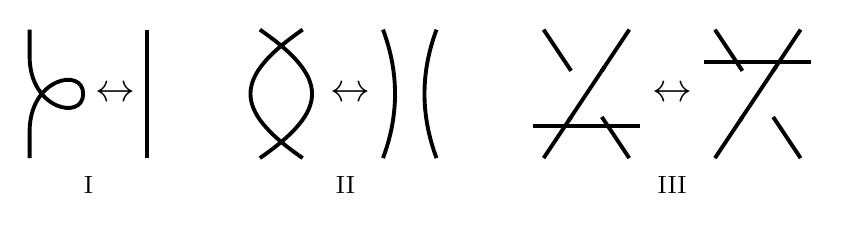
\begin{tikzpicture}[scale=0.68, every node/.style={font=\small}, line width=1.4pt]
  % Move I: a twist undone
  \begin{knot}[consider self intersections, clip width=4]
    \strand (0,0) -- (0,0.5) .. controls (0,1.5) and (1,1.7) .. (1,1.2) .. controls (1,0.7) and (0,0.9) .. (0,1.9) -- (0,2.4);
  \end{knot}
  \draw (2.2,0) -- (2.2,2.4);
  % Move II: two strands that cross twice pulled apart
  \begin{knot}[clip width=4]
    \strand (4.3,0) .. controls (5.6,0.9) and (5.6,1.5) .. (4.3,2.4);
    \strand (5.1,0) .. controls (3.8,0.9) and (3.8,1.5) .. (5.1,2.4);
  \end{knot}
  \draw (6.6,0) .. controls (6.9,0.8) and (6.9,1.6) .. (6.6,2.4) (7.6,0) .. controls (7.3,0.8) and (7.3,1.6) .. (7.6,2.4);
  % Move III: the top strand slides from below the crossing to above it
  \begin{knot}[clip width=4]
    \strand (9.4,0.6) -- (11.4,0.6);
    \strand (9.6,0) -- (11.2,2.4);
    \strand (11.2,0) -- (9.6,2.4);
  \end{knot}
  \begin{knot}[clip width=4]
    \strand (12.6,1.8) -- (14.6,1.8);
    \strand (12.8,0) -- (14.4,2.4);
    \strand (14.4,0) -- (12.8,2.4);
  \end{knot}
  \foreach \x/\n in {1.1/I, 5.9/II, 12/III} \node at (\x,-0.5) {\n};
  \foreach \x in {1.6, 6, 12} \node[font=\Large] at (\x,1.2) {$\leftrightarrow$};
\end{tikzpicture}
